% ================================================================
%  NUCLEO-G474RE POWER ELECTRONICS GUIDE
%  CONTRIBUTOR TEMPLATE  --  Version 1.0
% ================================================================
%
%  HOW TO USE THIS FILE
%  ───────────────────────────────────────────────────────────────
%  This template documents every convention used across Projects
%  01--06. Read the inline comments before filling any section.
%  Guidance text that must be replaced is wrapped in
%  \textit{[Guidance: ...]} so it is visible in the rendered PDF.
%
%  QUICK START
%  1. Duplicate this file and rename it:  NN_ProjectName.tex
%     where NN is the two-digit project number (07, 08, ...).
%
%  2. In CUSTOM COMMANDS below, update:
%       \newcommand{\projecttitle}{ ... }
%       \newcommand{\projectnumber}{ NN }
%       \newcommand{\projectdescription}{ ... }
%
%  3. In HEADER AND FOOTER, update:
%       \lhead{\textit{Project NN: YourTitle}}
%
%  4. On the title page, update the framework line:
%       STM32CubeIDE only  |  MATLAB only  |  Both
%
%  5. Work through each section top to bottom, replacing all
%     \textit{[Guidance: ...]} blocks with real content.
%
%  6. Compile twice:  pdflatex NN_ProjectName.tex  (twice for TOC)
%
%  IMAGE PATH CONVENTION
%  ───────────────────────────────────────────────────────────────
%  All images must live under the project subfolder:
%    NN_ProjectName/CUBE_IDE/imagename.png    (CubeIDE screenshots)
%    NN_ProjectName/MATLAB_Coder/imagename.png (Simulink screenshots)
%    NN_ProjectName/config/imagename.png       (CubeMX config screenshots)
%  Use:  \includegraphics[width=0.85\textwidth]{NN_Folder/sub/name.png}
%
%  CAPTION RULE (strictly enforced)
%  ───────────────────────────────────────────────────────────────
%  Captions must be 45 words or fewer. Describe:
%    (1) the component or screen shown,
%    (2) its role in the system, and
%    (3) one non-obvious detail the reader cannot see immediately.
%  Do NOT repeat information already in the surrounding paragraph.
%
%  TIKZ REUSE GUIDE
%  ───────────────────────────────────────────────────────────────
%  Two reference TikZ diagrams are provided in the Overview
%  section: an MCU execution flow and a framework comparison.
%  To adapt them for your project:
%    - Add/remove \node entries and matching \draw arrows.
%    - Use  proc=stateBlue  for main-flow steps (blue),
%           proc=isrGreen   for ISR / callback steps (green),
%           proc=btnOrange  for event / interrupt steps (orange).
%    - Use \node[decision] for branching diamonds.
%    - Use \node[terminal] for start/end pills.
%    - For landscape diagrams, wrap in \begin{landscape}...\end{landscape}
%      (requires \usepackage{lscape}).
%
%  FRAMEWORK SELECTION GUIDE
%  ───────────────────────────────────────────────────────────────
%  Include Section 2 (STM32CubeIDE) if your project has a
%  manual C firmware path.
%  Include Section 3 (MATLAB Embedded Coder) if your project
%  uses Simulink / model-based design.
%  If only one framework is used, DELETE the unused section and
%  adjust the title page framework line accordingly.
%  (Projects 01--05 use both; Project 06 uses MATLAB only.)
% ================================================================

\documentclass[11pt,a4paper,oneside]{article}

% ============= PACKAGES =============
\usepackage[T1]{fontenc}
\usepackage[margin=1in, headheight=14pt]{geometry}
\usepackage{graphicx}
\usepackage{amsmath}
\usepackage{amssymb}
\usepackage{listings}
\usepackage{xcolor}
\usepackage{hyperref}
\usepackage{fancyhdr}
\usepackage{titlesec}
\usepackage{tocloft}
\usepackage{array}
\usepackage{tabularx}
\usepackage{float}
\usepackage{subcaption}
\usepackage{cite}
\usepackage{url}
\usepackage{siunitx}
\usepackage{booktabs}
\usepackage{multirow}
\usepackage{tikz}
\usetikzlibrary{arrows.meta, shapes.geometric, shapes.misc,
                fit, backgrounds, calc, positioning}
\usepackage{lscape}   % for landscape TikZ diagrams (see Project 04)
% \usepackage{animate} % uncomment ONLY if embedding animated GIFs

% ============= COLOUR DEFINITIONS =============
% ── Brand colours ──────────────────────────────
\definecolor{stmblue}{RGB}{44, 123, 229}
\definecolor{darkblue}{RGB}{3, 35, 75}
% ── Code listing colours ───────────────────────
\definecolor{codegreen}{rgb}{0,0.6,0}
\definecolor{codegray}{rgb}{0.5,0.5,0.5}
\definecolor{codepurple}{rgb}{0.58,0,0.82}
\definecolor{codebackground}{rgb}{0.95,0.95,0.97}
% ── TikZ diagram palette ───────────────────────
%    Blue  = main-flow states / CubeIDE path
\definecolor{stateBlue}{RGB}{30,100,180}
\definecolor{stateFill}{RGB}{220,235,255}
%    Green = ISR / callback states / MATLAB path
\definecolor{isrGreen}{RGB}{20,130,80}
\definecolor{isrFill}{RGB}{210,245,225}
%    Orange = event / button / interrupt states
\definecolor{btnOrange}{RGB}{200,90,20}
\definecolor{btnFill}{RGB}{255,235,210}
%    Shared neutral colours
\definecolor{arrowGray}{RGB}{80,80,80}
\definecolor{labelColor}{RGB}{50,50,50}
\definecolor{decisionFill}{RGB}{255,250,200}
\definecolor{decisionBorder}{RGB}{180,150,0}
\definecolor{terminalFill}{RGB}{240,240,240}

% ============= FONT AND SPACING =============
\usepackage{setspace}
\onehalfspacing

\titleformat{\section}
  {\normalfont\Large\bfseries\color{darkblue}}
  {\thesection}{1em}{}

\titleformat{\subsection}
  {\normalfont\large\bfseries\color{stmblue}}
  {\thesubsection}{1em}{}

\titleformat{\subsubsection}
  {\normalfont\normalsize\bfseries}
  {\thesubsubsection}{1em}{}

% ============= CODE LISTINGS CONFIGURATION =============
% Available language values: C, MATLAB, bash, Python
% Add  morekeywords={HAL_GPIO_WritePin,...}  to extend keyword highlighting.
\lstset{
    backgroundcolor=\color{codebackground},
    commentstyle=\color{codegreen},
    keywordstyle=\color{codepurple}\bfseries,
    numberstyle=\tiny\color{codegray},
    stringstyle=\color{codepurple},
    basicstyle=\ttfamily\small,
    breakatwhitespace=false,
    breaklines=true,
    captionpos=b,
    keepspaces=true,
    numbers=left,
    numbersep=5pt,
    showspaces=false,
    showstringspaces=false,
    showtabs=false,
    tabsize=2,
    frame=single,
    rulecolor=\color{lightgray},
    xleftmargin=10pt,
    xrightmargin=5pt
}

% ============= HEADER AND FOOTER =============
\pagestyle{fancy}
\fancyhf{}
\rhead{\textcolor{stmblue}{NUCLEO-G474RE Power Electronics Guide}}
% UPDATE \lhead for every new project:
\lhead{\textit{Project NN: Your Title Here}}
\cfoot{\thepage}
\renewcommand{\headrulewidth}{0.5pt}
\renewcommand{\footrulewidth}{0pt}
\fancypagestyle{plain}{
  \fancyhf{}
  \cfoot{\thepage}
}

% ============= CUSTOM COMMANDS =============
% UPDATE these three commands for every new project.
\newcommand{\projecttitle}{Your Project Title}
\newcommand{\projectnumber}{NN}
\newcommand{\projectdescription}{One-sentence description of what this project demonstrates.}

\newcommand{\stmtitle}[1]{\textcolor{darkblue}{\textbf{#1}}}
\newcommand{\codetitle}[1]{\textit{\textcolor{stmblue}{#1}}}

% Highlighted note box (blue border, light blue fill)
% Usage: \note{This is an important note.}
\newcommand{\note}[1]{
  \vspace{0.5em}
  \noindent\fcolorbox{stmblue}{blue!5}{
    \parbox{0.96\textwidth}{
      \textbf{\textcolor{darkblue}{Note:}} #1
    }
  }
  \vspace{0.5em}
}

% Bulleted prerequisite line (blue bullet, italic text)
% Usage: \prerequisite{MATLAB R2025a with Embedded Coder installed}
\newcommand{\prerequisite}[1]{
  \vspace{0.3em}
  \noindent\textcolor{stmblue}{$\bullet$} \textit{#1}
}

% ============= DOCUMENT START =============
\begin{document}

% ============= TITLE PAGE =============
% The title page is fixed in layout. Update only the three
% \newcommand values above and the framework line below.
\begin{titlepage}
    \centering

    \vspace*{2cm}

    {\Huge \bfseries \textcolor{darkblue}{NUCLEO-G474RE}}

    \vspace{0.5cm}

    {\LARGE \textcolor{stmblue}{Power Electronics Project Series}}

    \vspace{2cm}

    {\fontsize{24}{28}\selectfont \bfseries Project \projectnumber}

    \vspace{1.5cm}

    {\Large \projecttitle}

    \vspace{2cm}

    {\large \projectdescription}

    \vspace{3cm}

    {\normalsize
        % Choose ONE of the three lines below and delete the others:
        %   Both frameworks:
        \textbf{Implementation Frameworks:}\\
        STM32CubeIDE \quad $\mid$ \quad MATLAB Embedded Coder
        %   MATLAB only (e.g. Project 06):
        % \textbf{Implementation Framework:}\\
        % MATLAB Embedded Coder \& Simulink
        %   CubeIDE only:
        % \textbf{Implementation Framework:}\\
        % STM32CubeIDE
    }

    \vspace{4cm}

    {\footnotesize
        Document Version: 1.0\\
        Last Updated: \today
    }

    \vfill

    {\small
        \textcolor{gray}{
            GitHub: \url{https://github.com/Anmol-G-K/NUCLEO-G474RE-PowerElectronics-Guide}\\
            This work is licensed under the MIT License
        }
    }

\end{titlepage}

% ============= TABLE OF CONTENTS =============
\newpage
\tableofcontents
\newpage

% ================================================================
%  SECTION 1 — PROJECT OVERVIEW
% ================================================================
\section{Project Overview}

% ── OBJECTIVE ───────────────────────────────────────────────────
% Keep this to 35 words maximum. State what the project does,
% which peripheral or algorithm is demonstrated, and on which
% framework. Do NOT repeat the project title word-for-word.
\subsection{Objective}

\textit{[Guidance: State the project goal in 35 words or fewer.
Example --- ``This project implements closed-loop PI control of a
buck converter using MATLAB/Simulink and the STM32G474RE ADC/DAC.
The architecture splits plant and controller across the PC and
the embedded target.'']}

% ── APPLICATIONS ────────────────────────────────────────────────
\subsection{Applications}

\textit{[Guidance: List 3--5 real-world domains or use cases
where this technique is applied. Be specific; avoid generic
statements like ``useful in industry.'']}

\begin{itemize}
    \item \textit{Application 1 --- describe concisely.}
    \item \textit{Application 2 --- describe concisely.}
    \item \textit{Application 3 --- describe concisely.}
\end{itemize}

% ── KEY CONCEPTS ────────────────────────────────────────────────
% Always include the domain concepts (Power Electronics, Digital
% Controls) plus one project-specific concept.
\subsection{Key Concepts}

\begin{itemize}
    \item \textbf{Power Electronics:} \textit{[Guidance: Name the
    topology, switching device, or conversion principle involved,
    e.g.\ ``Buck converter, duty-cycle control, CCM operation.'']}

    \item \textbf{Digital Control Systems:} \textit{[Guidance:
    Name the control law, discretisation method, or relevant
    concept, e.g.\ ``PI controller, anti-windup, Tustin
    discretisation.'']}

    \item \textbf{Embedded Firmware / Model-Based Design:}
    \textit{[Guidance: Describe the MCU-specific concept
    demonstrated, e.g.\ ``DMA-driven ADC sampling, HRTIM
    complementary PWM, or Simulink hardware deployment.'']}
\end{itemize}

% ── LEARNING OUTCOMES ───────────────────────────────────────────
\subsection{Learning Outcomes}

By completing this project, you will:

\begin{itemize}
    \item \textit{Outcome 1 --- begin with a verb, e.g.\ ``Understand
    how timer prescaler and ARR set the PWM switching frequency.''}
    \item \textit{Outcome 2.}
    \item \textit{Outcome 3.}
    \item \textit{Outcome 4 (optional).}
\end{itemize}

% ── REFERENCE DIAGRAM 1: MCU EXECUTION ARCHITECTURE ─────────────
% This TikZ diagram shows the generic STM32 execution model.
% It is provided as a REFERENCE. Adapt it for your project by:
%   - Renaming states to match your ISR callbacks.
%   - Adding extra ISR branches if needed.
%   - Removing the background-tasks branch for MATLAB-only projects.
% Colour key: blue = main flow, green = ISR/callback, orange = events.
\subsection{Overall Execution Architecture}

The diagram below illustrates the generic execution model shared
by all projects in this series. Every project follows this
pattern: hardware initialisation, an idle main loop, and
interrupt-driven callbacks for time-critical operations.

\begin{figure}[H]
\centering
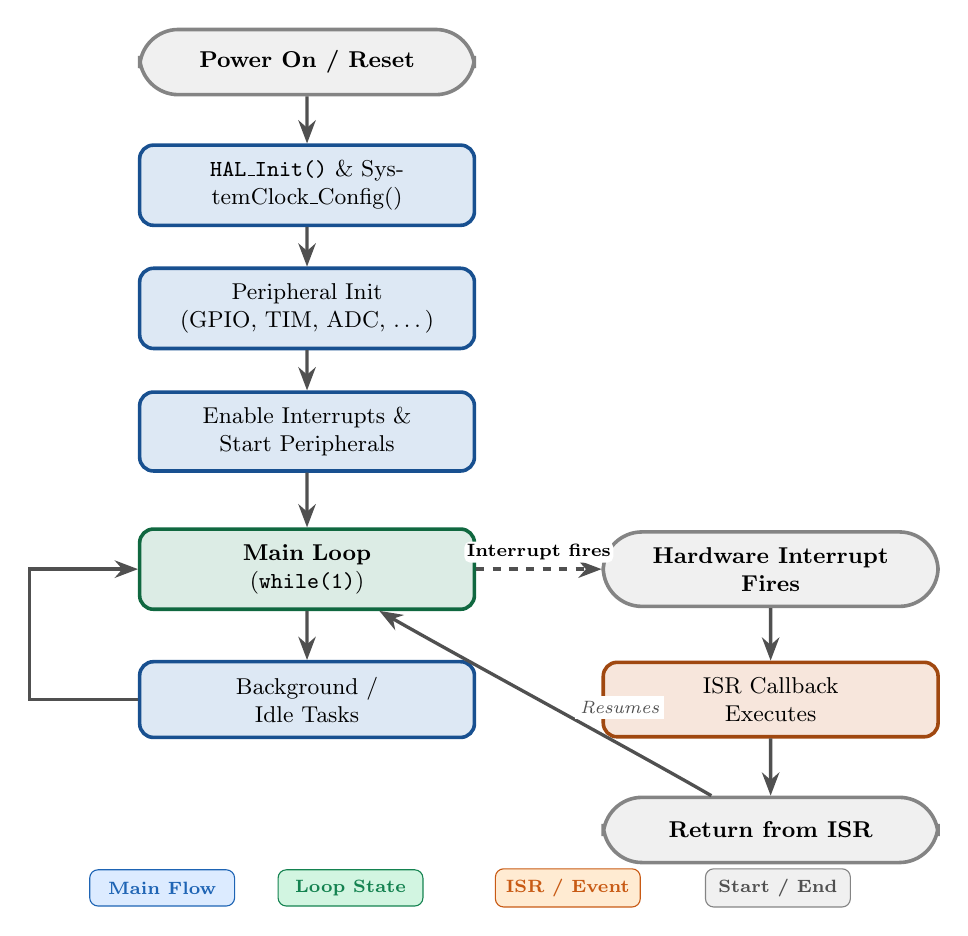
\begin{tikzpicture}[
    scale=0.92, transform shape,
    >=Stealth,
    % Parameterised process block: \node[proc=COLOR] or \node[proc]
    proc/.style={
        rectangle, rounded corners=5pt,
        draw=#1!80!black, fill=#1!15,
        line width=1.3pt,
        text width=4.2cm, align=center,
        minimum height=0.95cm,
        font=\small, inner sep=6pt
    },
    proc/.default=stateBlue,
    % Decision diamond
    decision/.style={
        diamond, aspect=2.2,
        draw=decisionBorder, fill=decisionFill,
        line width=1.3pt,
        text width=2.6cm, align=center,
        font=\small\itshape, inner sep=3pt
    },
    % Start / end pill
    terminal/.style={
        rectangle, rounded corners=14pt,
        draw=arrowGray!70, fill=terminalFill,
        line width=1.3pt,
        text width=4.2cm, align=center,
        minimum height=0.9cm,
        font=\small\bfseries, inner sep=6pt
    },
    lbl/.style={font=\scriptsize\bfseries, fill=white,
                inner sep=1pt, rounded corners=2pt},
    nolbl/.style={font=\scriptsize\itshape, text=arrowGray,
                  fill=white, inner sep=2pt}
]
% ── LEFT COLUMN: main execution path ──────────────────────────
\node[terminal]        (start)   at (0,   0.0) {Power On / Reset};
\node[proc]            (halinit) at (0,  -1.7) {\texttt{HAL\_Init()} \&\
                                                SystemClock\_Config()};
\node[proc]            (periph)  at (0,  -3.4) {Peripheral Init\\
                                                (GPIO, TIM, ADC, \ldots)};
\node[proc]            (irqen)   at (0,  -5.1) {Enable Interrupts \&\\
                                                Start Peripherals};
\node[proc=isrGreen]   (loop)    at (0,  -7.0) {\textbf{Main Loop}\\
                                                (\texttt{while(1)})};
\node[proc]            (bg)      at (0,  -8.8) {Background /\\
                                                Idle Tasks};
% ── RIGHT COLUMN: interrupt path ──────────────────────────────
\node[terminal]        (isrfire) at (6.4, -7.0) {Hardware Interrupt\\
                                                  Fires};
\node[proc=btnOrange]  (isrcb)   at (6.4, -8.8) {ISR Callback\\
                                                  Executes};
\node[terminal]        (isrret)  at (6.4,-10.6) {Return from ISR};
% ── ARROWS: main column ───────────────────────────────────────
\draw[-Stealth, line width=1.2pt, draw=arrowGray]
    (start)  -- (halinit);
\draw[-Stealth, line width=1.2pt, draw=arrowGray]
    (halinit) -- (periph);
\draw[-Stealth, line width=1.2pt, draw=arrowGray]
    (periph) -- (irqen);
\draw[-Stealth, line width=1.2pt, draw=arrowGray]
    (irqen)  -- (loop);
\draw[-Stealth, line width=1.2pt, draw=arrowGray]
    (loop)   -- (bg);
% Return from background tasks back to main loop (left L-path)
\draw[-Stealth, line width=1.2pt, draw=arrowGray]
    (bg.west) -- ++(-1.5,0) |- (loop.west);
% ── ARROWS: interrupt path ────────────────────────────────────
% Dashed horizontal line: interrupt fires from within main loop
\draw[-Stealth, line width=1.2pt, draw=arrowGray, dashed]
    (loop.east) -- node[lbl, above=2pt] {Interrupt fires} (isrfire.west);
\draw[-Stealth, line width=1.2pt, draw=arrowGray]
    (isrfire) -- (isrcb);
\draw[-Stealth, line width=1.2pt, draw=arrowGray]
    (isrcb)   -- (isrret);
% Curved return arrow: ISR completes, resumes main loop
\draw[-Stealth, line width=1.2pt, draw=arrowGray]
    (isrret) to[out=150, in=-30, looseness=0.55]
    node[nolbl, right=8pt, pos=0.48] {Resumes} (loop);
% ── Legend ────────────────────────────────────────────────────
\node[draw=stateBlue,  fill=stateFill,  rounded corners=3pt,
      font=\scriptsize\bfseries, text=stateBlue,
      inner sep=4pt, minimum width=2.0cm, minimum height=0.5cm]
    at (-2.0,-11.4) {Main Flow};
\node[draw=isrGreen,   fill=isrFill,    rounded corners=3pt,
      font=\scriptsize\bfseries, text=isrGreen,
      inner sep=4pt, minimum width=2.0cm, minimum height=0.5cm]
    at ( 0.6,-11.4) {Loop State};
\node[draw=btnOrange,  fill=btnFill,    rounded corners=3pt,
      font=\scriptsize\bfseries, text=btnOrange,
      inner sep=4pt, minimum width=2.0cm, minimum height=0.5cm]
    at ( 3.6,-11.4) {ISR / Event};
\node[draw=arrowGray!70, fill=terminalFill, rounded corners=3pt,
      font=\scriptsize\bfseries, text=arrowGray,
      inner sep=4pt, minimum width=2.0cm, minimum height=0.5cm]
    at ( 6.5,-11.4) {Start / End};
\end{tikzpicture}
\caption{Generic STM32 execution model: hardware initialises once, then the main loop runs indefinitely. Hardware interrupts preempt the loop, execute an ISR callback atomically, then return control. Background tasks run during idle periods between interrupts.}
\label{fig:exec_model}
\end{figure}

% ── REFERENCE DIAGRAM 2: FRAMEWORK COMPARISON ────────────────────
% This diagram shows the two development paths used across this
% series. It can be reused as-is or removed if your project uses
% only one framework. No changes needed unless you want to add
% extra workflow steps to a column.
\subsection{Development Framework Paths}

This series supports two complementary development paths.
Figure~\ref{fig:framework} summarises how each route reaches
the same validated embedded target.

\begin{figure}[H]
\centering
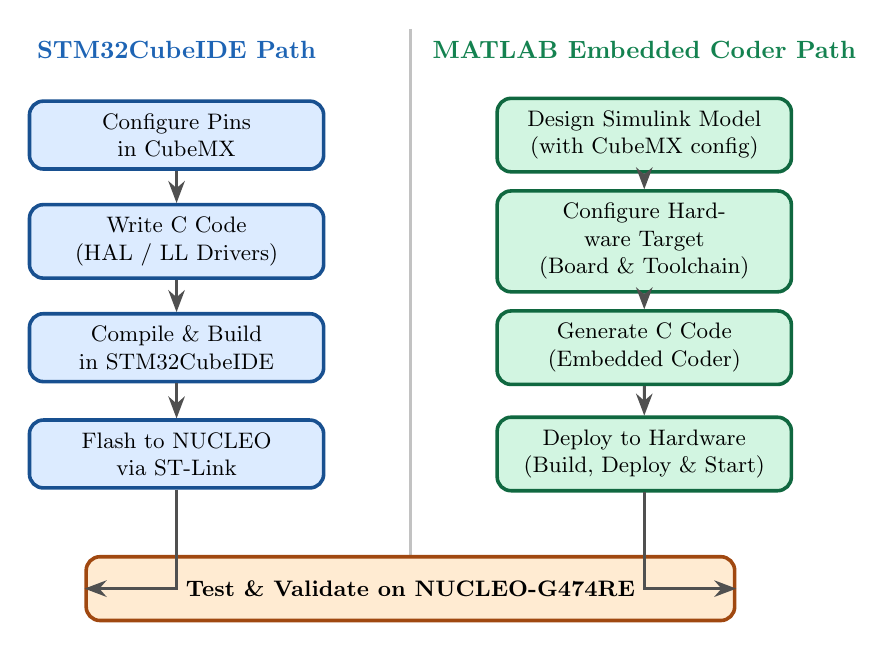
\begin{tikzpicture}[
    scale=0.90, transform shape,
    >=Stealth,
    % Blue block (CubeIDE path)
    procB/.style={
        rectangle, rounded corners=5pt,
        draw=stateBlue!80!black, fill=stateFill,
        line width=1.3pt,
        text width=3.8cm, align=center,
        minimum height=0.9cm,
        font=\small, inner sep=5pt
    },
    % Green block (MATLAB path)
    procG/.style={
        rectangle, rounded corners=5pt,
        draw=isrGreen!80!black, fill=isrFill,
        line width=1.3pt,
        text width=3.8cm, align=center,
        minimum height=0.9cm,
        font=\small, inner sep=5pt
    },
    % Orange shared block (common to both)
    procO/.style={
        rectangle, rounded corners=5pt,
        draw=btnOrange!80!black, fill=btnFill,
        line width=1.3pt,
        text width=8.8cm, align=center,
        minimum height=0.9cm,
        font=\small\bfseries, inner sep=5pt
    }
]
% Column headers
\node[font=\normalsize\bfseries, text=stateBlue]
    at (-3.3, 0.6) {STM32CubeIDE Path};
\node[font=\normalsize\bfseries, text=isrGreen]
    at ( 3.3, 0.6) {MATLAB Embedded Coder Path};
% Vertical divider
\draw[draw=arrowGray!35, line width=0.8pt] (0, 0.9) -- (0, -7.0);
% ── CubeIDE steps (left, x = -3.3) ──────────────────────────
\node[procB] (c1) at (-3.3, -0.6) {Configure Pins in CubeMX};
\node[procB] (c2) at (-3.3, -2.1) {Write C Code\\(HAL / LL Drivers)};
\node[procB] (c3) at (-3.3, -3.6) {Compile \& Build\\in STM32CubeIDE};
\node[procB] (c4) at (-3.3, -5.1) {Flash to NUCLEO\\via ST-Link};
% ── MATLAB steps (right, x = 3.3) ────────────────────────────
\node[procG] (m1) at (3.3, -0.6) {Design Simulink Model\\(with CubeMX config)};
\node[procG] (m2) at (3.3, -2.1) {Configure Hardware Target\\(Board \& Toolchain)};
\node[procG] (m3) at (3.3, -3.6) {Generate C Code\\(Embedded Coder)};
\node[procG] (m4) at (3.3, -5.1) {Deploy to Hardware\\(Build, Deploy \& Start)};
% ── Common convergence ────────────────────────────────────────
\node[procO] (common) at (0, -7.0)
    {Test \& Validate on NUCLEO-G474RE};
% ── Arrows: CubeIDE column ───────────────────────────────────
\draw[-Stealth, line width=1.1pt, draw=arrowGray] (c1) -- (c2);
\draw[-Stealth, line width=1.1pt, draw=arrowGray] (c2) -- (c3);
\draw[-Stealth, line width=1.1pt, draw=arrowGray] (c3) -- (c4);
% c4 to common: go down then route to common.west
\draw[-Stealth, line width=1.1pt, draw=arrowGray]
    (c4.south) |- (common.west);
% ── Arrows: MATLAB column ────────────────────────────────────
\draw[-Stealth, line width=1.1pt, draw=arrowGray] (m1) -- (m2);
\draw[-Stealth, line width=1.1pt, draw=arrowGray] (m2) -- (m3);
\draw[-Stealth, line width=1.1pt, draw=arrowGray] (m3) -- (m4);
% m4 to common: go down then route to common.east
\draw[-Stealth, line width=1.1pt, draw=arrowGray]
    (m4.south) |- (common.east);
\end{tikzpicture}
\caption{Dual-framework development paths: STM32CubeIDE (blue, left) follows manual C firmware development whilst MATLAB Embedded Coder (green, right) uses model-based code generation. Both paths converge at the same NUCLEO-G474RE target for validation.}
\label{fig:framework}
\end{figure}

% ── PNG IMAGE PLACEHOLDER ────────────────────────────────────────
% When your project has a system architecture diagram, a wiring
% diagram, or any high-level overview image, place it here.
% Use this placeholder pattern -- replace the \fbox block with
% \includegraphics once your PNG is ready.
%
% CAPTION GUIDANCE (max 45 words):
%   State (1) what the diagram shows, (2) the two or three main
%   components and how they connect, (3) the data-flow direction.
%   Example 45-word caption:
%   "System architecture: STM32G474RE controller (right) receives
%    simulated output voltage via USART3, outputs it through the
%    DAC, and reads it back through the ADC via a jumper wire.
%    Duty cycle is transmitted to the PC-side Simscape plant via
%    LPUART1."
%
% PNG SIZE GUIDANCE:
%   - System / wiring diagrams: width=0.85\textwidth
%   - CubeMX configuration screenshots: width=0.80\textwidth
%   - Side-by-side screenshots: use \begin{subfigure} pairs at
%     width=0.48\textwidth each (see Projects 05 and 06 for examples)
%   - High-resolution diagrams you created externally (e.g. block
%     diagrams exported from draw.io): width=0.85\textwidth to
%     0.92\textwidth so detail remains legible.
%
\begin{figure}[H]
    \centering
    % ── REPLACE THIS BLOCK WITH YOUR IMAGE ───────────────────
    \fbox{\parbox{0.85\textwidth}{\centering\vspace{2.8cm}
        \textcolor{stmblue}{\Large\bfseries [ SYSTEM ARCHITECTURE PNG ]}\\[0.6em]
        \small Replace with: \texttt{\textbackslash includegraphics%
        [width=0.85\textbackslash textwidth]\{NN\_Folder/system\_architecture.png\}}\\[0.4em]
        \textit{Use for: overall system block diagram, wiring diagram,
        or any high-level architectural overview image. Check the below image for an example.}
        \vspace{1cm}}}
    % ─────────────────────────────────────────────────────────
    \vspace{0.5cm} % Adjust this value to change the spacing between the box and the image

    % ── ACTUAL EXAMPLE IMAGE ─────────────────────────────────
    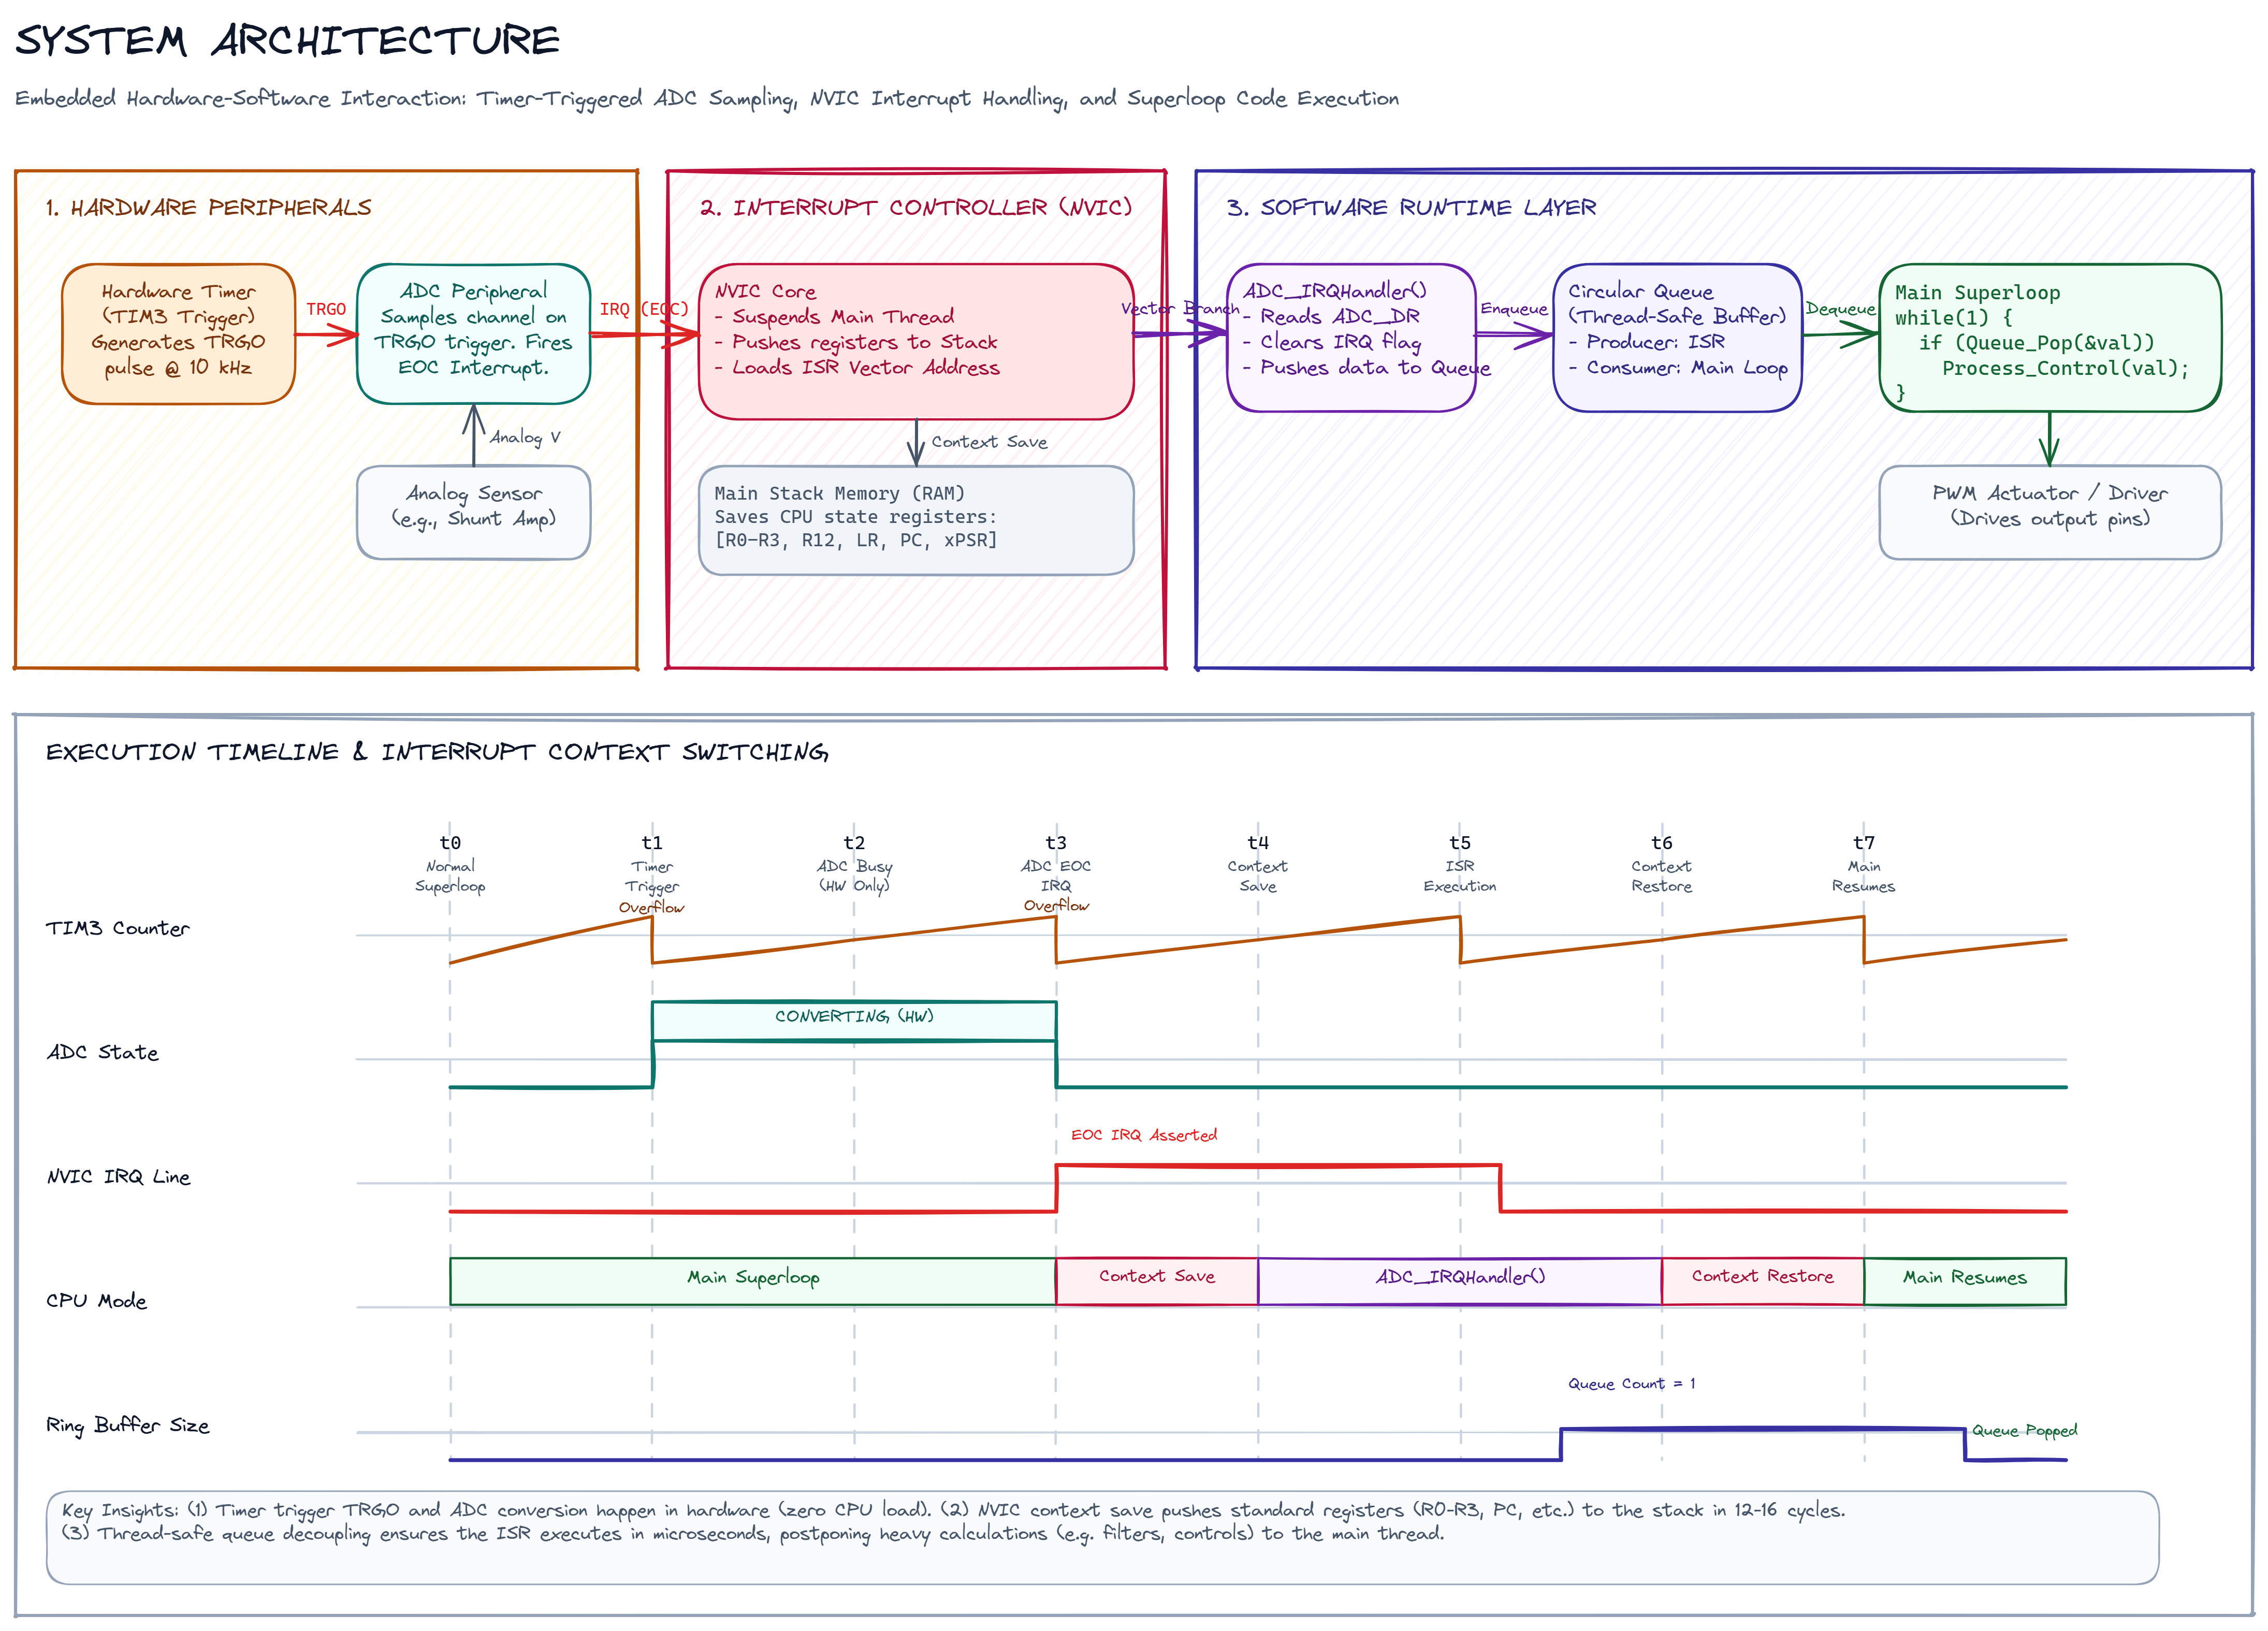
\includegraphics[width=0.85\textwidth]{embedded_workflow.png}
    
    \caption{\textit{[Guidance: Write your caption here, max 45 words.
    Describe the main components shown, their interconnections, and the
    direction of data flow. Do not repeat what is already stated in the
    surrounding paragraph text.]}}
    \label{fig:system_architecture}
\end{figure}

% ================================================================
%  SECTION 2 — STM32CUBEIDE IMPLEMENTATION
% ================================================================
% DELETE this entire section if your project is MATLAB-only.
\section{STM32CubeIDE Implementation}

\subsection{Prerequisites}

Before starting this implementation, ensure you have completed
the previous projects in this series, available at
\href{https://github.com/Anmol-G-K/NUCLEO-G474RE-PowerElectronics-Guide/tree/main/Examples}{the project repository}.

\prerequisite{STM32CubeIDE version 1.10 or later installed}
\prerequisite{NUCLEO-G474RE development board and USB cable}
\prerequisite{Completion of Projects 01--\textit{NN-1} for foundational knowledge}
\prerequisite{\textit{[Guidance: Add any project-specific prerequisites, e.g.\
``Oscilloscope or logic analyser for PWM verification.'']}}

\subsection{Hardware Configuration}

\subsubsection{Pin Configuration}

% Add or remove rows as needed. Always include: Pin, Function, Description.
% Use \SI{}{} for frequencies and voltages, e.g. \SI{20}{kHz}.
\begin{table}[H]
    \centering
    \caption{Pin Configuration}
    \label{tab:pin_config_cube}
    \begin{tabularx}{\textwidth}{|l|l|X|}
        \hline
        \textbf{Pin} & \textbf{Function} & \textbf{Description} \\
        \hline
        PA5  & GPIO Output & On-board green LED (LD2) \\
        \hline
        PC13 & GPIO Input  & On-board user button (B1), falling-edge trigger \\
        \hline
        \textit{PXX} & \textit{Function} &
            \textit{[Guidance: Add your pin, e.g.\ ``ADC1 CH1 ---
            analogue input from potentiometer on PA0.'']} \\
        \hline
    \end{tabularx}
\end{table}

\note{Refer to the STM32G474RE Reference Manual (RM0440) for complete
pin definitions and electrical specifications. The NUCLEO-G474RE User
Manual (UM2505) documents morpho and Arduino connector pinouts.}

\subsubsection{Peripheral Configuration}

% Provide one subsection per peripheral used.
% Document: prescaler, ARR/period, resolution, clock source, DMA if used.
\textbf{\textcolor{stmblue}{Timer (TIMx):}}

\begin{table}[H]
    \centering
    \caption{TIMx Configuration --- \textit{[state purpose, e.g.\ ``20\,kHz PWM'']}}
    \label{tab:timer_config}
    \begin{tabularx}{\textwidth}{|l|X|}
        \hline
        \textbf{Parameter} & \textbf{Value and Rationale} \\
        \hline
        Clock Source    & Internal (\SI{170}{MHz} system clock) \\
        \hline
        Prescaler (PSC) & \textit{[value]} $\rightarrow$ Timer clock = \SI{170}{MHz} / (PSC+1) \\
        \hline
        Auto-Reload (ARR) & \textit{[value]} $\rightarrow$ Period = ARR ticks / timer clock \\
        \hline
        Mode            & \textit{[Up / Centre-aligned / etc.]} \\
        \hline
        Interrupt / DMA & \textit{[Enabled / Disabled and reason]} \\
        \hline
    \end{tabularx}
\end{table}

\textbf{\textcolor{stmblue}{Other Peripherals (ADC / DAC / UART / HRTIM):}}

\textit{[Guidance: For each additional peripheral, include a
similar table or a short paragraph describing resolution, sampling
rate, DMA channels, and any relevant clock-domain notes.
Reference the matching CubeMX screenshot in the MATLAB section
or Appendix.]}

\subsection{Software Architecture}

\subsubsection{Project Structure}

\begin{lstlisting}[language=bash, caption=STM32CubeIDE project directory layout]
NN_ProjectName/
|-- Core/
|   |-- Inc/
|   |   |-- main.h
|   |   `-- stm32g4xx_it.h
|   `-- Src/
|       |-- main.c            % Entry point; calls MX_xxx_Init()
|       |-- stm32g4xx_it.c    % ISR handlers (HAL callbacks here)
|       `-- <your_module>.c   % Project-specific logic
|-- Drivers/
|   `-- STM32G4xx_HAL_Driver/
`-- <ProjectName>.ioc         % CubeMX config (open to regenerate)
\end{lstlisting}

\subsubsection{Initialisation Flow}

\textit{[Guidance: Briefly describe the sequence of \texttt{MX\_xxx\_Init()}
calls generated by CubeMX and any custom setup performed after them.
One short paragraph is sufficient; the code listing below carries
the detail.]}

\subsection{Code Implementation}

\subsubsection{Peripheral Initialisation}

\begin{lstlisting}[language=C, caption=Key peripheral initialisation (auto-generated by CubeMX)]
/* USER CODE BEGIN 2 */
// Start TIMx in interrupt mode
HAL_TIM_Base_Start_IT(&htimX);

// Start ADC with DMA (if applicable)
HAL_ADC_Start_DMA(&hadcX, (uint32_t*)adc_buf, BUF_LEN);
/* USER CODE END 2 */
\end{lstlisting}

\subsubsection{Core Algorithm / Control Law}

% For longer functions, move the full listing to the Appendix and
% reference it here: "see Listing~\ref{lst:your_function}".
\begin{lstlisting}[language=C, caption=Core processing function]
// [Guidance: Paste the key function here.
//  Keep ISRs short; offload heavy computation to main loop via flags.]
void HAL_TIM_PeriodElapsedCallback(TIM_HandleTypeDef *htim)
{
    if (htim->Instance == TIM1)
    {
        // Time-critical action here (keep < 10 us for 20 kHz loops)
    }
}
\end{lstlisting}

\subsection{Building and Flashing}

\begin{enumerate}
    \item Open the \texttt{.ioc} file in STM32CubeMX; verify pin and
          peripheral settings match the tables above.
    \item Right-click project $\rightarrow$ \textbf{Build Project}.
          Resolve any compiler errors before proceeding.
    \item Connect the NUCLEO board via USB (ST-Link port).
    \item Right-click project $\rightarrow$ \textbf{Run As}
          $\rightarrow$ \textbf{STM32 C/C++ Application}.
\end{enumerate}

\note{If the board is not detected, install ST-Link USB drivers
from STMicroelectronics and try a different USB port.}

% ================================================================
%  SECTION 3 — MATLAB EMBEDDED CODER IMPLEMENTATION
% ================================================================
% DELETE this entire section if your project is CubeIDE-only.
\section{MATLAB Embedded Coder Implementation}

\subsection{Prerequisites}

Before starting this implementation, ensure you have completed
the previous projects at
\href{https://github.com/Anmol-G-K/NUCLEO-G474RE-PowerElectronics-Guide/tree/main/Examples}{the project repository}.

\prerequisite{MATLAB R2025a or later with Embedded Coder toolbox}
\prerequisite{Embedded Coder Support Package for STMicroelectronics STM32
              (install via Add-On Explorer)}
\prerequisite{ARM GCC Compiler configured in MATLAB --- change from default to
              \textbf{GNU Tools for ARM Embedded Processors}}
\prerequisite{NUCLEO-G474RE development board and USB cable}
\prerequisite{\textit{[Add any project-specific prerequisites here.]}}

\note{The ARM GCC compiler selection is critical. By default, MATLAB
uses a different toolchain; this must be changed to
\textbf{GNU Tools for ARM Embedded Processors} before the first
build attempt.}

\subsection{MATLAB/Simulink Model Design}

\subsubsection{Model Architecture}

\textit{[Guidance: Describe the top-level structure of your Simulink
model. List the main subsystems and their roles. State the sample
time and solver settings. For co-simulation projects (see Project 06),
explain the two-model split here.]}

\begin{itemize}
    \item \textbf{Input / Measurement subsystem:}
          \textit{[e.g.\ ADC read, signal scaling, sanity filtering.]}
    \item \textbf{Control Algorithm subsystem:}
          \textit{[e.g.\ PI controller, feedforward, gain scheduling.]}
    \item \textbf{Output / Actuation subsystem:}
          \textit{[e.g.\ PWM write, DAC output, UART transmit.]}
\end{itemize}

\subsubsection{Subsystem Summary}

\begin{table}[H]
    \centering
    \caption{Simulink subsystem descriptions}
    \label{tab:subsystems}
    \begin{tabularx}{\textwidth}{|l|X|}
        \hline
        \textbf{Subsystem / Block} & \textbf{Purpose} \\
        \hline
        \textit{Subsystem name} &
            \textit{[Guidance: One sentence describing what this
            subsystem does and why it is a separate block.]} \\
        \hline
        \textit{MATLAB Function: xxx} &
            \textit{[Guidance: Describe the codegen function; reference
            the Appendix listing, e.g.\ ``Implements the PI control
            law with anti-windup; see Appendix~A.'']} \\
        \hline
        \textit{ISR Block / Triggered Subsystem} &
            \textit{[Guidance: State which TIM or event triggers it
            and the sample period.]} \\
        \hline
    \end{tabularx}
\end{table}

% ── Peripheral Configuration (CubeMX screenshots) ───────────────
% Place CubeMX screenshots in pairs using subcaption, 0.48\textwidth each.
% Screenshot path: NN_ProjectName/config/PERIPH-N.png
% Example pattern (used in Projects 05 and 06):
%
% \begin{figure}[H]
%     \centering
%     \begin{subfigure}[b]{0.48\textwidth}
%         \includegraphics[width=\textwidth]{NN_Folder/config/ADC-1.png}
%         \caption{ADC channel and resolution settings.}
%     \end{subfigure}
%     \hfill
%     \begin{subfigure}[b]{0.48\textwidth}
%         \includegraphics[width=\textwidth]{NN_Folder/config/ADC-2.png}
%         \caption{ADC DMA channel configuration.}
%     \end{subfigure}
%     \caption{ADC1 configuration in CubeMX. (Max 45 words total.)}
%     \label{fig:adc_config}
% \end{figure}

\subsection{Model Configuration}

\subsubsection{Solver Settings}

\begin{itemize}
    \item \textbf{Solver Type:} Fixed-step
    \item \textbf{Solver:} Discrete (no continuous states)
          --- use \textit{ode3 (Bogacki-Shampine)} only for Simscape models
    \item \textbf{Fixed Step Size:} \textit{[e.g.\ \texttt{1/20000}
          for a \SI{20}{kHz} control loop]}
\end{itemize}

\subsubsection{Hardware Target Settings}

\textit{[Guidance: Confirm the following in Simulink Configuration
Parameters $\rightarrow$ Hardware Implementation:
Board: STM32G4xx based;
Toolchain: GNU Tools for ARM Embedded Processors;
External mode: off (unless using serial monitoring).]}

\subsection{Code Generation and Deployment}

\begin{enumerate}
    \item Press \textbf{Ctrl+E} to open Configuration Parameters.
          Verify board and toolchain settings.
    \item Connect the NUCLEO board via USB.
    \item In the Simulink toolbar, click
          \textbf{Deploy to Hardware} (Build, Deploy \& Start).
    \item MATLAB generates C code, compiles it with ARM GCC,
          and flashes the resulting binary via ST-Link.
\end{enumerate}

\note{Generated source files are placed in a folder named
\texttt{<ModelName>\_ert\_rtw/} next to the \texttt{.slx} file.
These are auto-generated; do not edit them directly.}

\subsection{MATLAB Functions (Codegen)}

% If your project uses MATLAB Function blocks with %#codegen,
% place full listings in the Appendix and reference them here.
% Keep this subsection to a short paragraph.
\textit{[Guidance: List each MATLAB Function block used (e.g.\
\texttt{buck\_controller.m}, \texttt{parse\_rx.m}), state its
inputs/outputs, and cross-reference its Appendix listing. Example:
``The control law is implemented in \texttt{buck\_controller}
(Appendix~\ref{app:code}). It accepts $V_\text{ref}$,
$V_o$, and $V_\text{in}$; returns duty ratio $D \in [0,\,0.95]$.'']}

% ================================================================
%  SECTION 4 — TESTING AND VALIDATION
% ================================================================
\section{Testing and Validation}

\subsection{Hardware Testing}

Before running the full system, verify each physical element:

\begin{enumerate}
    \item \textit{[Guidance: Step 1 --- verify power and connectivity,
          e.g.\ ``Confirm the board enumerates as a COM port.'']}
    \item \textit{[Guidance: Step 2 --- verify a key peripheral in
          isolation, e.g.\ ``Toggle PA5 manually in CubeIDE Live
          Expressions to confirm LED responds.'']}
    \item \textit{[Guidance: Step 3 --- verify signal chain,
          e.g.\ ``Probe PA8 with an oscilloscope; confirm
          \SI{20}{kHz} PWM at the expected duty cycle.'']}
\end{enumerate}

\subsection{Model Simulation Testing}

Before deploying to hardware, validate in Simulink simulation mode:

\begin{itemize}
    \item Replace hardware I/O blocks with step sources and scopes.
    \item Apply a step reference and verify the controller converges
          to setpoint within the expected settling time.
    \item Check that all saturation blocks activate only within
          their intended operating ranges.
\end{itemize}

\subsection{Integration Testing}

\textit{[Guidance: Describe 3--5 checks that confirm the full
hardware-software loop is working correctly. Include any checks
specific to your peripheral combination, e.g.\ DMA buffer
integrity, UART packet format, or ADC/DAC linearity.]}

% ================================================================
%  SECTION 5 — RESULTS AND ANALYSIS
% ================================================================
\section{Results and Analysis}

\subsection{Experimental Results}

% Include your result screenshots here. One paragraph per image,
% describing what it shows and what the expected value is.
% Example image block:
%
% \begin{figure}[H]
%     \centering
%     \includegraphics[width=0.80\textwidth]{NN_Folder/Output_Voltage.png}
%     \caption{Output voltage settling to approximately \SI{5}{V}.
%              Close-up view showing steady-state ripple of less than
%              \SI{50}{mV} peak-to-peak after the initial transient.}
%     \label{fig:output_voltage}
% \end{figure}

\textit{[Guidance: Include at minimum (a) a time-domain waveform
showing system response, (b) a steady-state result confirming
accuracy, and (c) optionally a PWM or hardware signal verification.
Follow the 45-word caption rule strictly.]}

\begin{table}[H]
    \centering
    \caption{Summary of experimental results}
    \label{tab:results}
    \begin{tabularx}{\textwidth}{|l|X|}
        \hline
        \textbf{Measurement} & \textbf{Value / Observation} \\
        \hline
        \textit{Parameter 1} & \textit{Result} \\
        \hline
        \textit{Parameter 2} & \textit{Result} \\
        \hline
        \textit{Parameter 3} & \textit{Result} \\
        \hline
    \end{tabularx}
\end{table}

\subsection{Key Observations}

\textit{[Guidance: 3--5 bullet points summarising the most
significant findings. Connect each observation back to a
specific result image or table above. End with one sentence
on any discrepancy between simulated and measured behaviour.]}

% ================================================================
%  SECTION 6 — TROUBLESHOOTING
% ================================================================
\section{Troubleshooting}

% Keep to 3--5 rows. Each issue must be specific and actionable.
% Avoid generic advice like "check all connections."
\begin{table}[H]
    \centering
    \caption{Common issues and solutions}
    \label{tab:troubleshooting}
    \begin{tabularx}{\textwidth}{|l|X|}
        \hline
        \textbf{Issue} & \textbf{Solution} \\
        \hline
        Code does not compile &
            Check that the correct board is selected in CubeMX and
            that all generated files are included in the build path \\
        \hline
        Board not detected &
            Install ST-Link drivers; try a different USB port;
            restart the IDE \\
        \hline
        MATLAB deploy fails &
            Confirm \textbf{GNU Tools for ARM Embedded Processors}
            is selected as the active toolchain \\
        \hline
        \textit{[Project-specific issue]} &
            \textit{[Concise, actionable solution.]} \\
        \hline
        \textit{[Project-specific issue]} &
            \textit{[Concise, actionable solution.]} \\
        \hline
    \end{tabularx}
\end{table}

% ================================================================
%  SECTION 7 — EXTENSIONS AND ENHANCEMENTS
% ================================================================
\section{Extensions and Enhancements}

\subsection{Possible Improvements}

% List 3--5 concrete, implementable extensions. Start each with
% a bold title, then a one-paragraph description. Close with
% a brief implementation hint.
\begin{enumerate}
    \item \textbf{\textit{[Enhancement 1 title]:}}
          \textit{[Guidance: Describe a concrete, implementable
          improvement. State what changes in hardware or software
          and what additional capability it provides. Close with
          one sentence on how to start.]}

    \item \textbf{\textit{[Enhancement 2 title]:}}
          \textit{[Guidance: Same structure.]}

    \item \textbf{\textit{[Enhancement 3 title]:}}
          \textit{[Guidance: Same structure.]}
\end{enumerate}

\subsection{Advanced Topics}

\begin{itemize}
    \item \textbf{FreeRTOS integration:} Replace the bare-metal
          superloop with a real-time OS to manage multiple
          concurrent control tasks with deterministic scheduling.
    \item \textbf{Multi-phase / multi-level topologies:} Extend the
          PWM and ADC configuration to support interleaved or
          cascaded converter stages.
    \item \textit{[Guidance: Add 1--2 advanced topics specific to
          your project domain.]}
\end{itemize}

% ================================================================
%  CONCLUSION
% ================================================================
\section{Conclusion}

\textit{[Guidance: Three to four sentences. State (1) what was
demonstrated, (2) which technique or peripheral was the key
contribution, (3) the primary limitation or open question, and
(4) how this project builds toward the next one in the series.
Do NOT say ``this project successfully demonstrated'' --- start
with the actual result.]}

\textbf{Key Takeaways:}

\begin{itemize}
    \item \textit{[Takeaway 1: One sentence, specific to this project.]}
    \item \textit{[Takeaway 2: One sentence.]}
    \item \textit{[Takeaway 3: One sentence on tool selection or
          framework trade-off learned.]}
\end{itemize}

% ================================================================
%  REFERENCES
% ================================================================
\newpage

\begin{thebibliography}{99}

% These four references are common to all projects. Do not remove.
\bibitem{ref:g474re_manual}
STMicroelectronics, \textit{STM32G4 Series Advanced ARM-based
32-bit MCUs Reference Manual}, RM0440.

\bibitem{ref:g474re_datasheet}
STMicroelectronics, \textit{STM32G474RE Datasheet}.

\bibitem{ref:nucleo_manual}
STMicroelectronics, \textit{STM32G4 NUCLEO-64 Boards User
Manual}, UM2505.

\bibitem{ref:hal_drivers}
STMicroelectronics, \textit{Description of STM32G4 HAL and
Low-Layer Drivers}, UM2570.

% Add project-specific references below. Use this format:
% \bibitem{ref:shortname}
% Author(s) or Organisation, \textit{Title}, Publisher/Source,
% Year (if known).
\bibitem{ref:embedded_coder}
MathWorks, \textit{Embedded Coder Documentation}.

\bibitem{ref:ec_stm32_support}
MathWorks, \textit{Embedded Coder Support Package for
STMicroelectronics STM32}.

\bibitem{ref:hrtim_cookbook}
STMicroelectronics, \textit{HRTIM Cookbook}, AN4539.
% ── Add project-specific references here ──────────────────────

\end{thebibliography}

% ================================================================
%  APPENDICES
% ================================================================
\newpage
\appendix

% ── APPENDIX A: Full Code Listings ──────────────────────────────
% Place complete MATLAB function listings here.
% Reference in-text as: Appendix~\ref{app:your_function}
% Keep function comments concise. Remove redundant inline comments
% before pasting (the code should be self-documenting at this level).
\section{Code Listings}
\label{app:code}

\textit{[Guidance: Place full MATLAB function code, helper
utilities, or any code too long for the main body here. Use
a separate \texttt{\textbackslash subsection} per function. Use the
\texttt{[language=Matlab]} or \texttt{[language=C]} option in
\texttt{\textbackslash begin\{lstlisting\}}.]}

\begin{lstlisting}[language=Matlab, caption=\texttt{your\_function.m} --- brief one-line description]
function output = your_function(input1, input2)
%#codegen
% Brief description: what this computes and why.
% Inputs:  input1 - description [units / range]
%          input2 - description [units / range]
% Outputs: output - description [units / range]

% Implementation here
output = input1 + input2;
end
\end{lstlisting}

% ── APPENDIX B: CubeMX / Hardware Configuration Screenshots ─────
% If CubeMX screenshots are too numerous for the main body,
% place them here. Reference as: Appendix~\ref{app:cubemx}
\section{Peripheral Configuration Screenshots}
\label{app:cubemx}

\textit{[Guidance: Move any CubeMX screenshots that would
interrupt the flow of the main text here. Use the paired
\texttt{\textbackslash subfigure} pattern at 0.48\texttt{\textbackslash textwidth} each.]}

% ── APPENDIX C: Hardware Documentation ──────────────────────────
\section{Hardware Documentation}

Refer to the official NUCLEO-G474RE schematic and the STM32G474RE Reference
Manual (RM0440) for complete hardware specifications, electrical
characteristics, and pin definitions.

% ================================================================
%  AUTHOR AND ACKNOWLEDGMENTS
% ================================================================
\newpage
\section*{Author}

\textbf{Anmol Govindarajapuram Krishnan}

GitHub: \url{https://github.com/Anmol-G-K}

Email: cb.en.u4eee23103@cb.students.amrita.edu

\section*{Acknowledgments}

\begin{itemize}
    \item \textbf{STMicroelectronics} for comprehensive MCU
          documentation and development tools
    \item \textbf{MathWorks} for MATLAB and Embedded Coder resources
    \item The embedded systems and power electronics community
          for knowledge sharing and innovation
    \item Contributors and reviewers providing feedback on
          this project series
\end{itemize}

This project is licensed under the MIT License.

\vspace{1cm}

\noindent\textit{For updates and additional resources:}

\noindent\url{https://github.com/Anmol-G-K/NUCLEO-G474RE-PowerElectronics-Guide}

\end{document}